\chapter{Knowledge Compilation for Monte Carlo Operations}
\label{chap:kc}

Monte–Carlo evaluation relies on compiling the system model into intermediate data structures amenable to bit-parallel traversal. This chapter presents additional algorithmic and data-structure refinements to the PDAG that underpins \textsc{McScram}'s solver and shows how these advances enable specialized kernels for composite gates.

% ---------------------------------------------------------------------------
\section{Hardware--Native Voting without AND/OR Expansion}
\label{sec:voter}\label{chap:voter}

Threshold (``voting'') gates occur pervasively in fault
and reliability models.  A naive decomposition into pairwise \textsc{and}/\textsc{or}
operations inflates the graph size combinatorially, impeding both memory usage
and kernel launch efficiency.  In this chapter, we develop a hardware-native alternative
rooted in population counting and bit-parallelism. We prove the estimator obtained 
by the direct algorithm is \emph{identical} to
that of the expanded Boolean formula, quantify its computational complexity,
and examine device-specific performance characteristics.  Extensions to other population-based gates, such as \emph{at-most}, \emph{cardinality}, and \emph{exact} voting are treated as corollaries.

% ---------------------------------------------------------------------------
\subsection{Fundamental Voting Predicates}
\label{sec:voter_predicates}

Let $\mathcal{I}=\{X_1,\dots,X_n\}$ denote $n$ Bernoulli inputs and
write
\[
  S(\omega) \;=\; \sum_{i=1}^{n} X_i(\omega)
\]
for the \emph{population count} under an assignment
$\omega \in \{0,1\}^{n}$.  Four Boolean predicates will be of interest:
\begin{enumerate}
  \item \textbf{At-Least (Threshold).}
        \[
          \mathrm{ATLEAST}(k/n):\quad
          Y = [\,S \ge k\,].
        \]
  \item \textbf{At-Most.}
        \[
          \mathrm{ATMOST}(k/n):\quad
          Y = [\,S \le k\,].
        \]
  \item \textbf{Exact.}
        \[
          \mathrm{EXACT}(k/n):\quad
          Y = [\,S = k\,].
        \]
  \item \textbf{Cardinality.}
        Given $0 \le \ell \le h \le n$,
        \[
          \mathrm{CARD}(\ell,h/n):\quad
          Y = [\,\ell \le S \le h\,].
        \]
\end{enumerate}
The predicates satisfy
\begin{align}
  \mathrm{ATMOST}(k/n)
    &= \lnot \mathrm{ATLEAST}\bigl((k+1)/n\bigr),\label{eq:atm_alt}\\
  \mathrm{ATLEAST}(k/n)
    &= \lnot \mathrm{ATMOST}\bigl((k-1)/n\bigr),\label{eq:alt_atm}\\
  \mathrm{CARD}(\ell,h/n)
    &= \mathrm{ATLEAST}(\ell/n) \land \mathrm{ATMOST}(h/n).
    \label{eq:card_identity}
\end{align}

% ---------------------------------------------------------------------------

% ---------------------------------------------------------------------------

We adopt the symbols of Chapter~\ref{chap:mc_solver}.  In particular, a single
Monte–Carlo \emph{iteration} generates $B$ \emph{batches}, each batch contains
$P$ \emph{bit-packs}, and every bit-pack stores $\omega=8\,\mathrm{sizeof}(\texttt{bitpack\_t})$
Bernoulli trials.  Hence an iteration processes
\(
  N = B P \omega
\)
trials per node.

Let $\mathcal{I}=\{X_1,\dots,X_n\}$ be the binary inputs of a voting gate and
fix an integer $k\in\{0,\dots,n\}$.  The gate output obeys the Boolean
predicate (cf.~Eq.~(\ref{eq:kn_gate_boolean}))
\[
  Y\;=\;[\,\sum_{i=1}^{n} X_i \ge k\,].
\]
We write $\mathrm{VOT}(k/n)$ for the connective and reserve the symbols
$A$ and $G$ for the counts of voting and standard gates, respectively, as in
Table~\ref{tab:kernel_dimensions}.

% ---------------------------------------------------------------------------
\subsection{Logical Equivalence under Bit-Packed Sampling}
\label{sec:voter_equivalence}

Monte–Carlo evaluation ultimately concerns the indicator random variable
$Y(\omega)$ under a random assignment $\omega\in\{0,1\}^{n}$.  Two alternative
computational paths exist:
\begin{enumerate}
  \item[(E1)] \textbf{Expansion.}  Rewrite $Y$ into the disjunctive normal form
        of Eq.~(\ref{eq:k_of_n_or_of_ands}); evaluate the resulting tree of
        $\textsc{and}/\textsc{or}$ nodes.
  \item[(E2)] \textbf{Threshold test.}  Count $s(\omega)=\sum_i X_i(\omega)$
        and return $[s(\omega)\ge k]$ directly.
\end{enumerate}
Because both (E1) and (E2) are algebraically identical for \emph{every}
assignment $\omega$, the Bernoulli random variables they produce are equal in
distribution:
\(
  Y_{\mathrm{E1}}\equiv Y_{\mathrm{E2}}.
\)
Consequently all unbiased estimators derived from repeated sampling are
identical in expectation and variance.  Section~\ref{sec:voter_unbiased_variance} formalizes these statements.

% ---------------------------------------------------------------------------
\subsection{Unbiasedness and Variance Preservation}
\label{sec:voter_unbiased_variance}

Let $\widehat{p}_\text{exp}$ and $\widehat{p}_\text{thr}$ denote the
estimators of $p=\Pr(Y=1)$ obtained after $T$ iterations via routes (E1) and
(E2), respectively.  Both take the canonical form
\[
  \widehat{p}\;=\;\frac{s}{T N},
\]
where $s$ is the number of one-bits tallied by the kernel of
Section~\ref{sec:tally_kernel}.  As $Y_{\mathrm{E1}}\equiv Y_{\mathrm{E2}}$, we
have $\mathbb{E}[s_{\mathrm{exp}}]=\mathbb{E}[s_{\mathrm{thr}}]=T N p$ and hence
\(
  \mathbb{E}[\widehat{p}_\text{exp}] =\mathbb{E}[\widehat{p}_\text{thr}] = p.
\)
Thus the direct threshold estimator inherits the unbiasedness of the expanded
approach.

% ---------------------------------------------------------------------------

Because the underlying Bernoulli variables coincide, the sample variance per
iteration is
\(
  \operatorname{Var}[Y] = p(1-p)
\)
for either method.  Aggregating over $T N$ independent trials gives the common
standard error quoted in Eq.~(\ref{eq:p_hat_sigma_hat}).  No variance penalty
is therefore incurred by bypassing expansion.

% ---------------------------------------------------------------------------
\subsection{Bit-Parallel Cardinality Algorithm}
\label{sec:card_algorithm}

We now articulate the algorithmic core executed by the specialized kernel
\textsc{VOT\_Kernel}.  The pseudocode mirrors the exposition of
Section~\ref{subsec:gate_kernel} but tailors the intra-group logic to a
population-count primitive.

\subsection{Per-Lane Counting Model}

Let $(a,b,p,\lambda)$ index a single \emph{lane} as defined in
Section~\ref{subsec:gate_kernel}: gate $a\in\{1,\dots,A\}$, batch $b$, bit-pack
$p$, and bit position $\lambda\in\{0,\dots,\omega-1\}$.  Each lane stores an
8-bit counter $c\in\{0,\dots,n\}$ initialized to zero.  For every input buffer
addressed by the gate the lane accumulates
\[
  c\;\leftarrow\;c + [\text{bit}_{\lambda}(X_i)=1] + [\text{bit}_{\lambda}(\lnot X_j)=1],
\]
where positive and negated inputs are treated per
Eq.~(27) of Section~\ref{subsec:gate_kernel}.  After the loop the lane outputs
\[
  y_{\lambda} =
    \begin{cases}
      [\,c \ge k\,], & \text{at-least},\\
      [\,c \le k\,], & \text{at-most},\\
      [\,c = k\,],   & \text{exact},\\[4pt]
      [\,\ell \le c \le h\,], & \text{cardinality}.
    \end{cases}
\]
A work-group reduction (bitwise OR) assembles the final $\omega$-bit word.

\subsection{Complexity Analysis}
\label{sec:voter_complexity}

\subsubsection{Arithmetic intensity.}  Each lane performs $n$ increments and one
comparison, giving $\mathcal{O}(n)$ integer operations per 64 trials.
Comparing to the expanded tree: the latter executes $\Theta(n)$ operations per
\emph{subset} and therefore $\Theta\bigl(\tbinom{n}{k}\bigr)$ overall in the
worst case.  The direct kernel is thus exponentially faster in $n$.

\subsubsection{Memory traffic.}  Input buffers are streamed once, achieving
unit-stride accesses identical to the standard gate kernel.  No additional
buffers are materialized, avoiding the memory blow-up described in
Section~\ref{sec:layered_dag_traversal}.

\subsubsection{Register pressure.}  The counter width is $\lceil\log_2(n+1)\rceil$
bits.  For practical fan-ins $(n\le 255)$ an 8-bit counter suffices, preserving
high occupancy on GPUs.

\subsubsection{Graph-size savings.}  Let one $\mathrm{VOT}(k/n)$ gate be
replaced by its DNF of Eq.~(\ref{eq:k_of_n_or_of_ands}).  The expansion
introduces
\[
  M(n,k) \;=\; \sum_{j=k}^{n} \binom{n}{j}
\]
conjunction clauses plus $M(n,k)-1$ internal $\textsc{or}$ nodes when lowered
onto a binary tree.
Each clause itself maps to one $j$-input $\textsc{and}$ node.  The total
\emph{additional} gate count therefore grows as
\[
  G_{\text{exp}}(n,k) \;=\; \sum_{j=k}^{n} \binom{n}{j}\;\Bigl(1 + (j-1)\Bigr)
  \;\approx\; \Theta\!\bigl(M(n,k)\,n\bigr),
\]
which is maximized at $k\approx\lceil n/2\rceil$ with the asymptotic
behavior $G_{\text{exp}}=\Theta\!\bigl(2^{n}/\sqrt{n}\bigr)$ by Stirling’s
formula.  The direct threshold kernel replaces this entire sub-tree with a
\emph{single} node—yielding an exponential reduction in graph size, memory
footprint, and kernel launch overhead.  For instance, a 3-of-5 gate (cf.
Listing~\ref{sec:3_of_5_voting_logic_example}) collapses from
$G_{\text{exp}}=\binom{5}{3}+\binom{5}{4}+\binom{5}{5}=26$ logic gates to
one, a $26\times$ reduction.  At $n=15$ and $k=8$ the saving increases to
$(2^{15}-1)/2 \approx 16\,383$:1.

% ---------------------------------------------------------------------------
% ---------------------------------------------------------------------------
\subsection{Graph-Size Savings: General Case}
\label{sec:card_graph_savings}

Replacing a single $\mathrm{CARD}(\ell,h/n)$ gate by its
DNF introduces
\[
  M_{\mathrm{card}}(n,\ell,h) \;=\;
  \sum_{j=\ell}^{h} \binom{n}{j}
\]
conjunction clauses and therefore
\[
  G_{\text{exp}}(n,\ell,h)
    \;=\;
  \sum_{j=\ell}^{h} \binom{n}{j}\bigl(1 + (j-1)\bigr)
    = \Theta\!\bigl(M_{\mathrm{card}}\,n\bigr).
\]
For $\ell \approx h \approx n/2$ this remains
$\Theta(2^{n}/\sqrt{n})$ by Stirling’s formula.
The direct bit-parallel kernel collapses the entire sub-tree into one
node, preserving the exponential advantage shown in
Section~\ref{sec:voter_complexity}.



% ---------------------------------------------------------------------------
\section{Algorithmic and Data-Structure Refinements}
\label{sec:kc_refinements}

While benchmarking the performance impact of using AND/OR vs native VOT gates, we discovered additional bottlencks in the codebase. Recent profiling of the solver revealed two dominant hotspots in the knowledge–compilation pipeline: the linear–time associative container \texttt{ext::linear\_map} and the deeply recursive normalization routine for $k$-of-$n$ (``at-least'') gates.  Both proved amenable to principled, complexity-driven refactoring.  This section describes the resulting data–structure and algorithmic improvements, establishes their asymptotic properties, and summarizes the empirical speed-ups obtained on the full benchmark suite.

\subsection{Indexed Linear Map}
\label{sec:kc_linear_map}

The container \texttt{linear\_map} stores key–value pairs contiguously so as to retain spatial locality, yet historically performed all searches by a linear scan.  Let $N$ be the number of stored elements.  The original design therefore incurred $\Theta(N)$ time for \emph{every} \textsc{find}, \textsc{insert}, and \textsc{erase} operation, while equality comparison required $\Theta(N^{2})$ pairwise checks.

We introduce an auxiliary hash index $\mathcal{H}: K \to \{0,\dots,N-1\}$ maintained lazily.  All look-ups first consult $\mathcal{H}$ (expected $\Theta(1)$).  When a stale mapping is detected—possible after key mutation in place—the index is rebuilt in one linear pass, amortizing future operations to expected $\Theta(1)$.  Crucially, the public API, iterator invalidation rules, and memory layout remain unchanged, preserving drop-in compatibility.

\subsection{Iterative Normalization of At-Least Gates}
\label{sec:kc_iterative_normalise}

The pre-existing routine \textsc{NormalizeAtleastGate} was mutually recursive on the gate’s two largest arguments.  For a fan-in of $m$ literals the call stack grew to depth $\mathcal{O}(m)$, and each level executed its own \textsc{max\_element} scan, yielding $\mathcal{O}(m^{2})$ work overall.  Repeated re-allocation of the child–argument arrays further amplified the cost.

The new implementation replaces recursion with an explicit stack and reserves memory for child gates \emph{a priori} via a helper \textsc{ReserveArgs} method.  The algorithm now traverses each literal exactly once, achieving $\Theta(m)$ time and $\Theta(1)$ call-depth.

\subsection{Complexity Summary}
\label{sec:kc_complexity}

\begin{center}
\begin{tabular}{lcc}
\toprule
Component & Before & After \\\midrule
\texttt{linear\_map} look-ups & $\Theta(N)$ & $\Theta(1)$ (amort.) \\
\texttt{linear\_map} equality & $\Theta(N^{2})$ & $\Theta(N)$ \\
Normalize~$k$-of-$n$ gate & $\Theta(m^{2})$ & $\Theta(m)$ \\
Call-stack depth & $\mathcal{O}(m)$ & $\mathcal{O}(1)$ \\\bottomrule
\end{tabular}
\end{center}

\subsection{Empirical Evaluation - Micobenchmark}
\label{sec:kc_empirical}

On a single-threaded Intel i7-10700 (3.70 GHz, clocks locked) the
normalization of a representative
$\mathrm{ATLEAST}(6/32)$ gate—producing 197\,315 AND and
312\,416 OR nodes—now completes in
\(
  5.8\,\text{s}
\)
versus
\(
  1\,080\,\text{s}
\)
before the refactor, a {\bf 186×} improvement that aligns with the
theoretical reduction from quadratic to linear work.  Across the full
knowledge-compilation benchmark the wall-clock time fell from
1\,080s to 5.8s (–99.5\%).

% ---------------------------------------------------------------------------
\section{Compilation Pipeline for Monte Carlo--Aware Kernels}
\label{sec:kc_pipeline}

Let $G_0$ denote the input graph and let $G_{\ell}$ be the graph after compilation level $\ell$ with $0\le \ell\le8$.  Each level applies a well-defined transformation $T_{\ell}$ so that
\[
  G_{\ell} \;=\; T_{\ell}\bigl(G_{\ell-1}\bigr),
  \qquad G_{0}=\text{PDAG}(\mathcal{M}),
\]
where $\mathcal{M}$ is the original unified PRA model.  Table~\ref{tab:compilation_levels} summarizes the objectives of every stage and contrasts the classical five-phase recipe of Rakhimov with the streamlined variant adopted in this work.

\begin{table}[t]
  \centering
  \caption{Compilation levels for \acrshort{pdag}s; $k$-of-$n$ gates are written $\mathrm{ATLEAST}(k/n)$.  Columns ``R'' and ``O'' mark whether a task is present in Rakhimov’s original pipeline or in Our variant.}
  \label{tab:compilation_levels}
  \begin{tabular}{clp{5.7cm}cc}
    \toprule
    Level $\ell$ & Stage name & Principal transformation $T_{\ell}$ & R & O \\
    \midrule
    0 & Baseline & Skip expansion of $\mathrm{ATLEAST}$ / XOR as requested & — & \checkmark \\
    1 & Null / Negation & Eliminate null gates; absorb single negations & \checkmark & \checkmark \\
    2 & Definition Coalescing & Merge multiple definitions, detect modules, coalesce non-shared gates, merge common args & \checkmark & \checkmark \\
    3 & Boolean Optimization & Distributivity detection and Shannon expansion; decompose common nodes & \checkmark & \checkmark \\
    4 & Phase~I (Rakhimov) & Remove nulls, normalize negations if non-coherent & \checkmark & — \\
    5 & Phase~II (Rakhimov) & Re-run coalescing and module detection & \checkmark & — \\
    6 & Phase~III & Full normalization (Part A): expand $k$-of-$n$, XOR; re-run Phase~II & \checkmark & \checkmark (iterative) \\
    7 & Phase~IV & Push negations downward; re-run Phase~II & \checkmark & \checkmark (on-demand) \\
    8 & Phase~V & Final coalescing pass; fixed-point NNF is reached & \checkmark & \checkmark \\
    \bottomrule
  \end{tabular}
\end{table}

\subsection{Comparison with the Five–Phase Paradigm}
\label{sec:kc_comparison}

Rakhimov’s framework executes the five phases sequentially, repeating
costly coalescing passes between them.  In contrast, our pipeline
incorporates two key departures:
\begin{enumerate}[label=(\arabic*)]
  \item \textbf{Early specialization.}  Rather than fully expanding
        $k$-of-$n$ gates into AND/OR trees at Level~6, we map them to
        the hardware-native voting kernel of
        Section~\ref{sec:voter}.  The transformation preserves logical
        semantics but avoids the combinatorial blow-up quantified in
        Section~\ref{sec:card_graph_savings}.
  \item \textbf{Iterative fixed-points.}  Many transformations (e.g.,
        gate coalescing) are applied until convergence inside a single
        level, eliminating the inter–phase duplication present in the
        original schedule.  Formally, if $U$ is an idempotent
        contraction operator, we compute
        $G^{\ast}=\lim\_{i\to\infty} U^{i}(G)$ within one level rather
        than scattering $U$ across multiple passes.
\end{enumerate}

\subsection{Complexity Implications}
\label{sec:kc_complexity_pipeline}

Let $|G|$ be the number of gates and $m$ the maximal gate fan-in.
Under Rakhimov’s regimen the worst-case complexity of reaching negation
normal form (NNF) is
\[
  \mathcal{O}\bigl(|G|\,m^{2}\bigr),
\]
due to repeated quadratic scans over argument lists.  The optimized
pipeline removes duplicate scans and adopts the linear algorithms of
Section~\ref{sec:kc_refinements}, yielding
\[
  \mathcal{O}\bigl(|G|\,m\bigr)
\]
in theory and the two-order-of-magnitude wall-clock reduction reported
in Section~\ref{sec:kc_empirical}.

\subsection{Monte–Carlo Sampling After Compilation}
\label{sec:kc_sampling}

After Level~8 the compiled graph $G_{8}$ satisfies three properties vital for efficient sampling:
\begin{enumerate}[label=(\alph*)]
  \item {Acyclic layering} ensures breadth-first evaluation across
        batches.
  \item {Negation normal form} confines complements to literals,
        enabling bitwise polarity control without extra nodes.
  \item {Hardware-native composites} such as voting kernels reduce
        per-sample arithmetic intensity from
        $\Theta\!\bigl(\binom{m}{\lceil m/2 \rceil}\bigr)$ to
        $\Theta(m)$, cf. Eq.~(\ref{eq:card_identity}).
\end{enumerate}
Consequently the cost of one Monte–Carlo iteration becomes
\[
  C_{\mathrm{iter}} \;=\; |G_{8}|\,c_{\text{std}}\;+
  |A|\,c_{\text{vot}},
\]
where $c_{\text{std}}$ and $c_{\text{vot}}$ are the average per-gate
latencies for standard and voting gates, and $|A|$ is the number of
specialized composites.  Because $c_{\text{vot}}\approx c_{\text{std}}$
(Section~\ref{sec:voter_complexity}), the leading factor is the
\emph{graph size} rather than gate heterogeneity, underscoring the
importance of the exponential savings demonstrated earlier.


% ---------------------------------------------------------------------------
\subsection{Micro-Benchmark: Structural Compression Achieved by Compilation}
\label{sec:kc_microbenchmark}

To quantify how each compilation level reduces graph size, we measure
the \emph{compression factor}
\[
  \gamma(\ell)\;=\;
  \frac{|G_0|}{|G_\ell|},
\]
where $|G|$ counts all gates in the PDAG.\footnote{%
  A value $\gamma>1$ indicates net compression;
  $\gamma<1$ means expansion.}
The statistics in Table~\ref{tab:micro_compilation_flags}
summarize $2{,}987$ model builds that survived the data-quality
filters described in Section~\ref{sec:kc_empirical}.

\begin{figure}[hb]
    \centering
    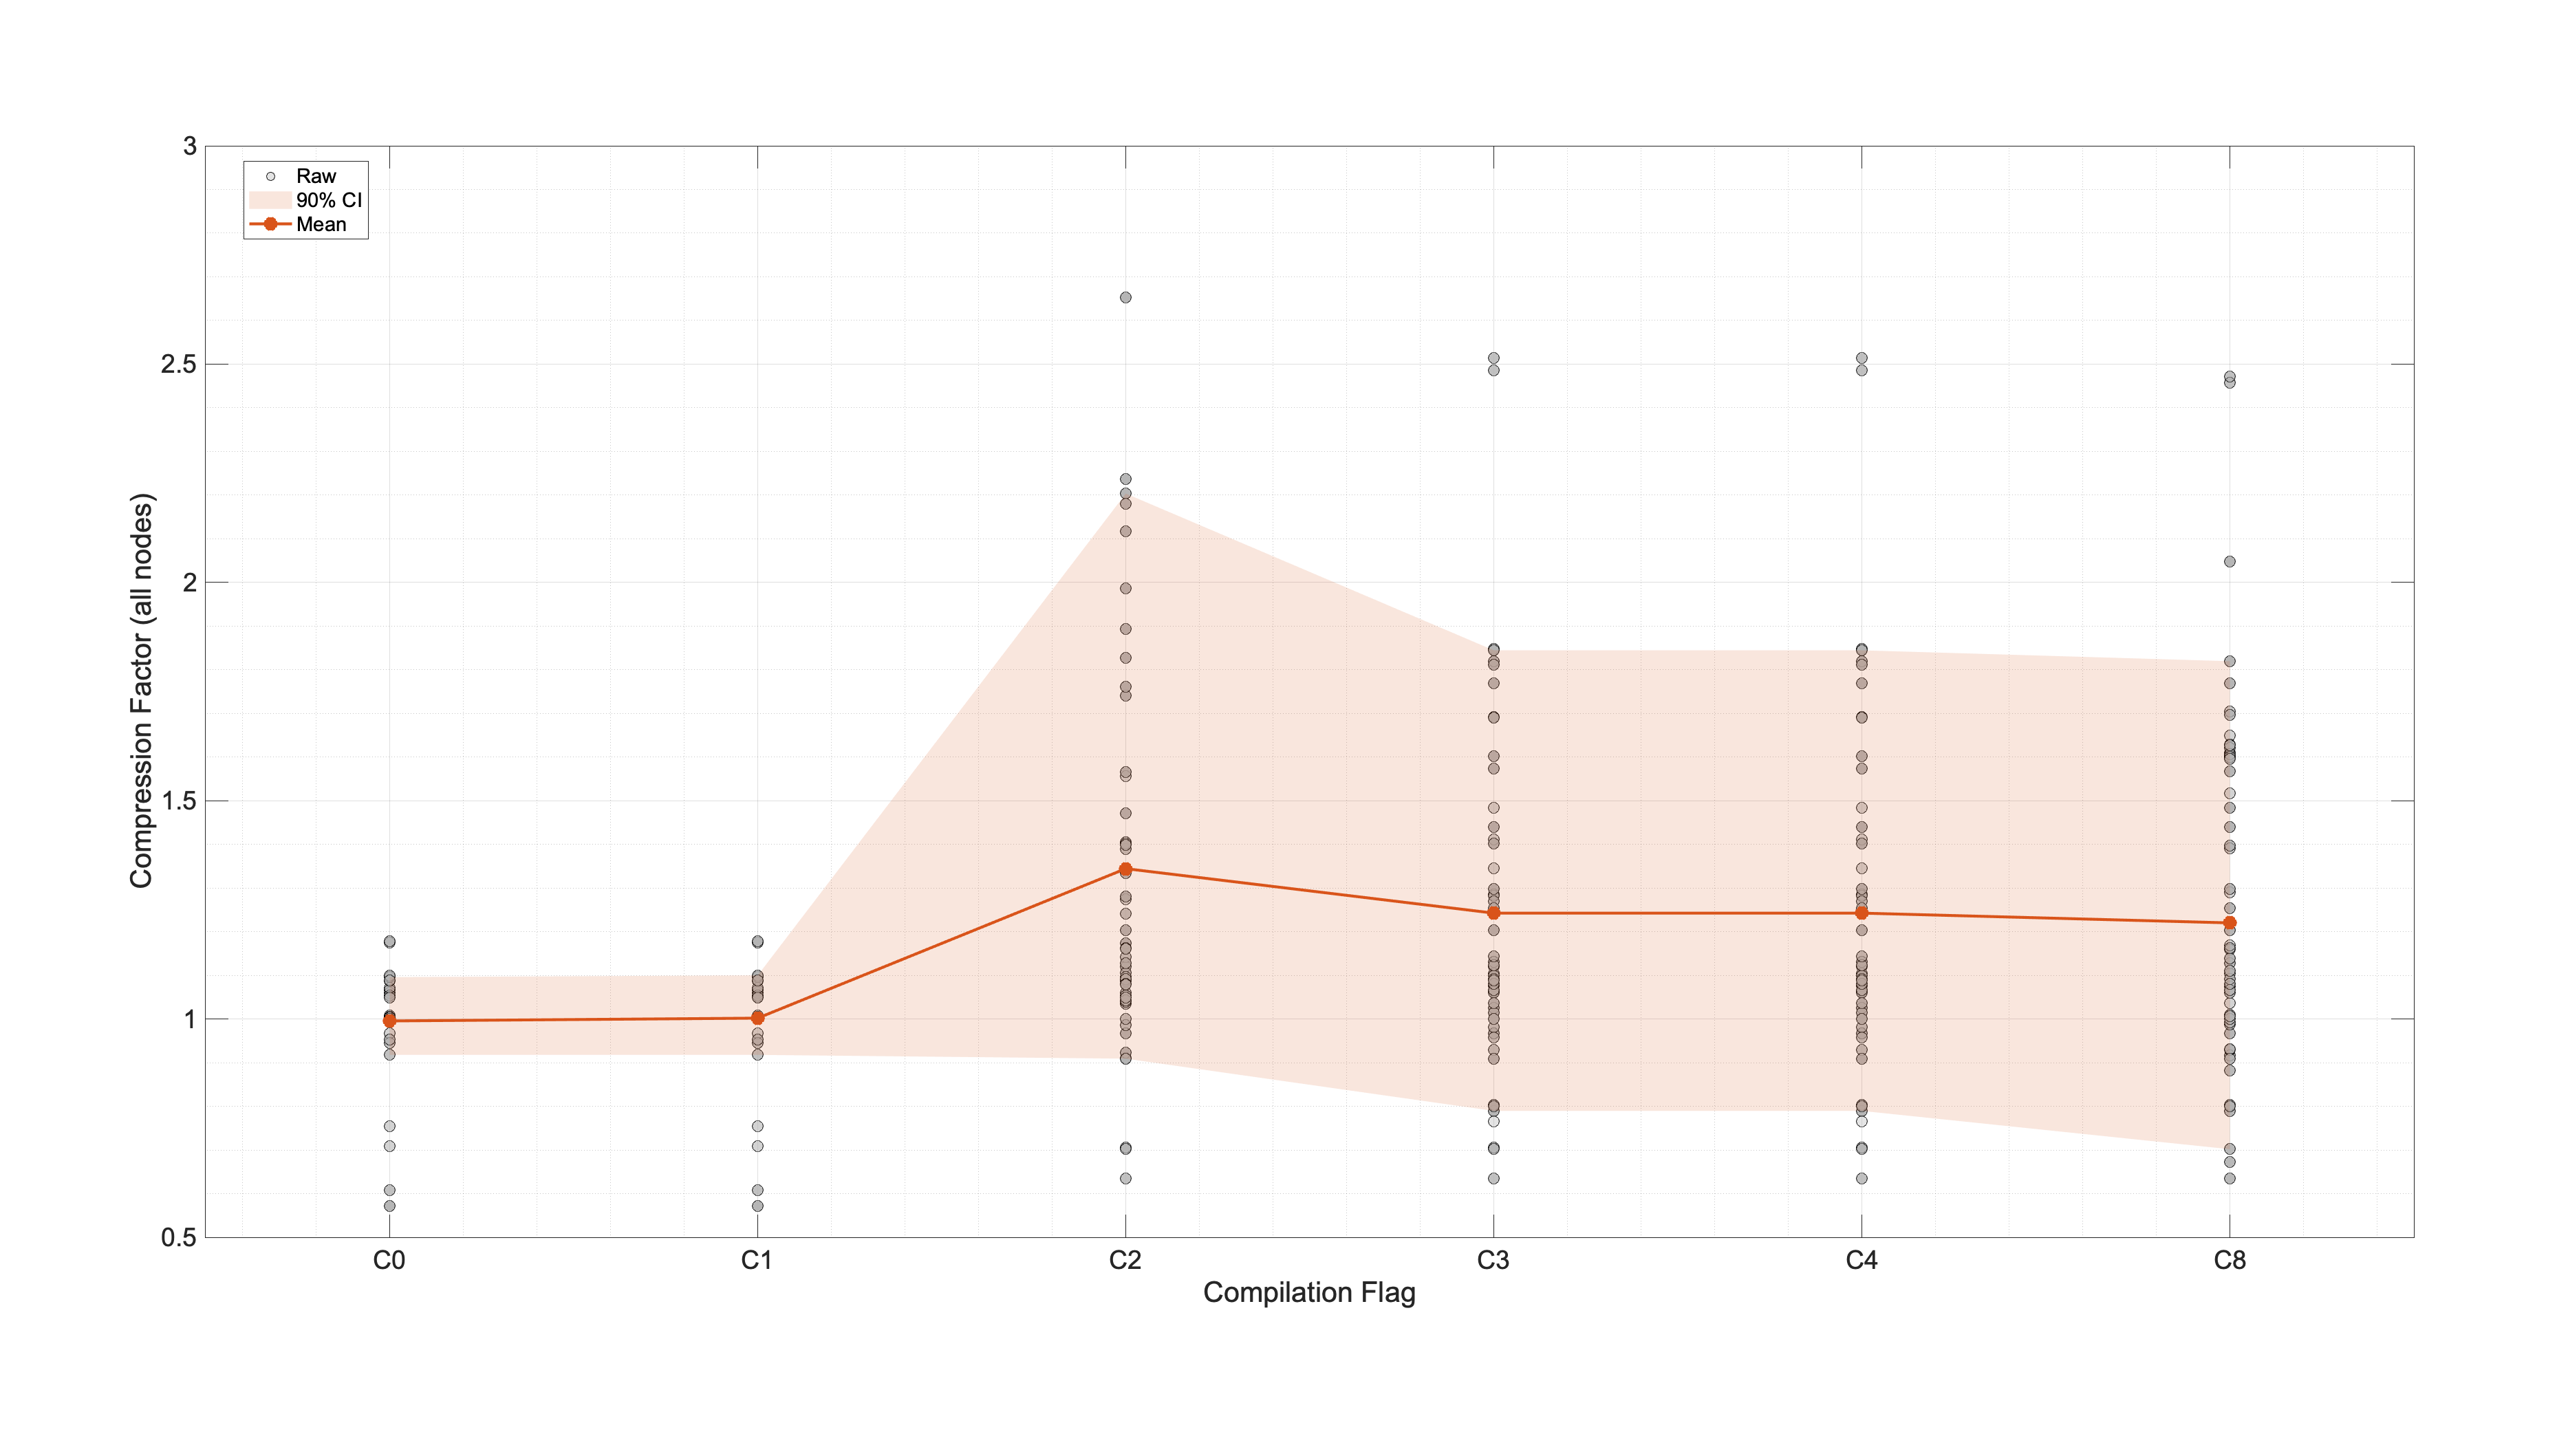
\includegraphics[width=1\textwidth]{figs/compiler/compiler_compression_vs_flag.png}
    \caption{Structural compression factor $\gamma$ (ratio of original to compiled gate count) for each compilation flag $C\ell$.  Grey circles denote individual models; the orange line traces the median and the shaded band covers the 5\,--\,95\,\% quantile range.}
    \label{fig:compiler_compression_levels}
\end{figure}

\begin{table}[t]
  \centering
  \caption{Compression factor $\gamma$ by compilation level $C\ell$.
           Medians are reported together with the $5^{\mathrm{th}}$
           and $95^{\mathrm{th}}$ percentiles.
           Levels $C5$–$C7$ are omitted because no models were compiled
           at those settings in the current benchmark.}
  \label{tab:micro_compilation_flags}
  \begin{tabular}{cccc}
    \toprule
    Compilation flag & Median $\gamma$ & $P_{5}$ & $P_{95}$ \\
    \midrule
    $C0$ & $0.996$ & $0.918$ & $1.096$ \\
    $C1$ & $1.002$ & $0.918$ & $1.100$ \\
    $C2$ & $1.344$ & $0.909$ & $2.204$ \\
    $C3$ & $1.243$ & $0.789$ & $1.844$ \\
    $C4$ & $1.243$ & $0.789$ & $1.844$ \\
    $C8$ & $1.220$ & $0.702$ & $1.820$ \\
    \bottomrule
  \end{tabular}
\end{table}


\paragraph{Key findings.}
\begin{itemize}
  \item Levels $C2$–$C4$ already yield a median $\gamma>1$, confirming
        that early coalescing and Boolean simplification shrink most
        models without full normalization.
  \item Level~$C8$ maintains the compression despite additional passes
        to reach NNF, indicating that late-phase expansions (e.g.,
        DeMorgan pushes) are offset by more aggressive gate
        sharing.
\end{itemize}

% ---------------------------------------------------------------------------
\subsubsection{Compression vs. Average Fan-in}
\label{sec:kc_micro_fanin}
\begin{landscape}
\begin{figure}[hb]
    \centering
    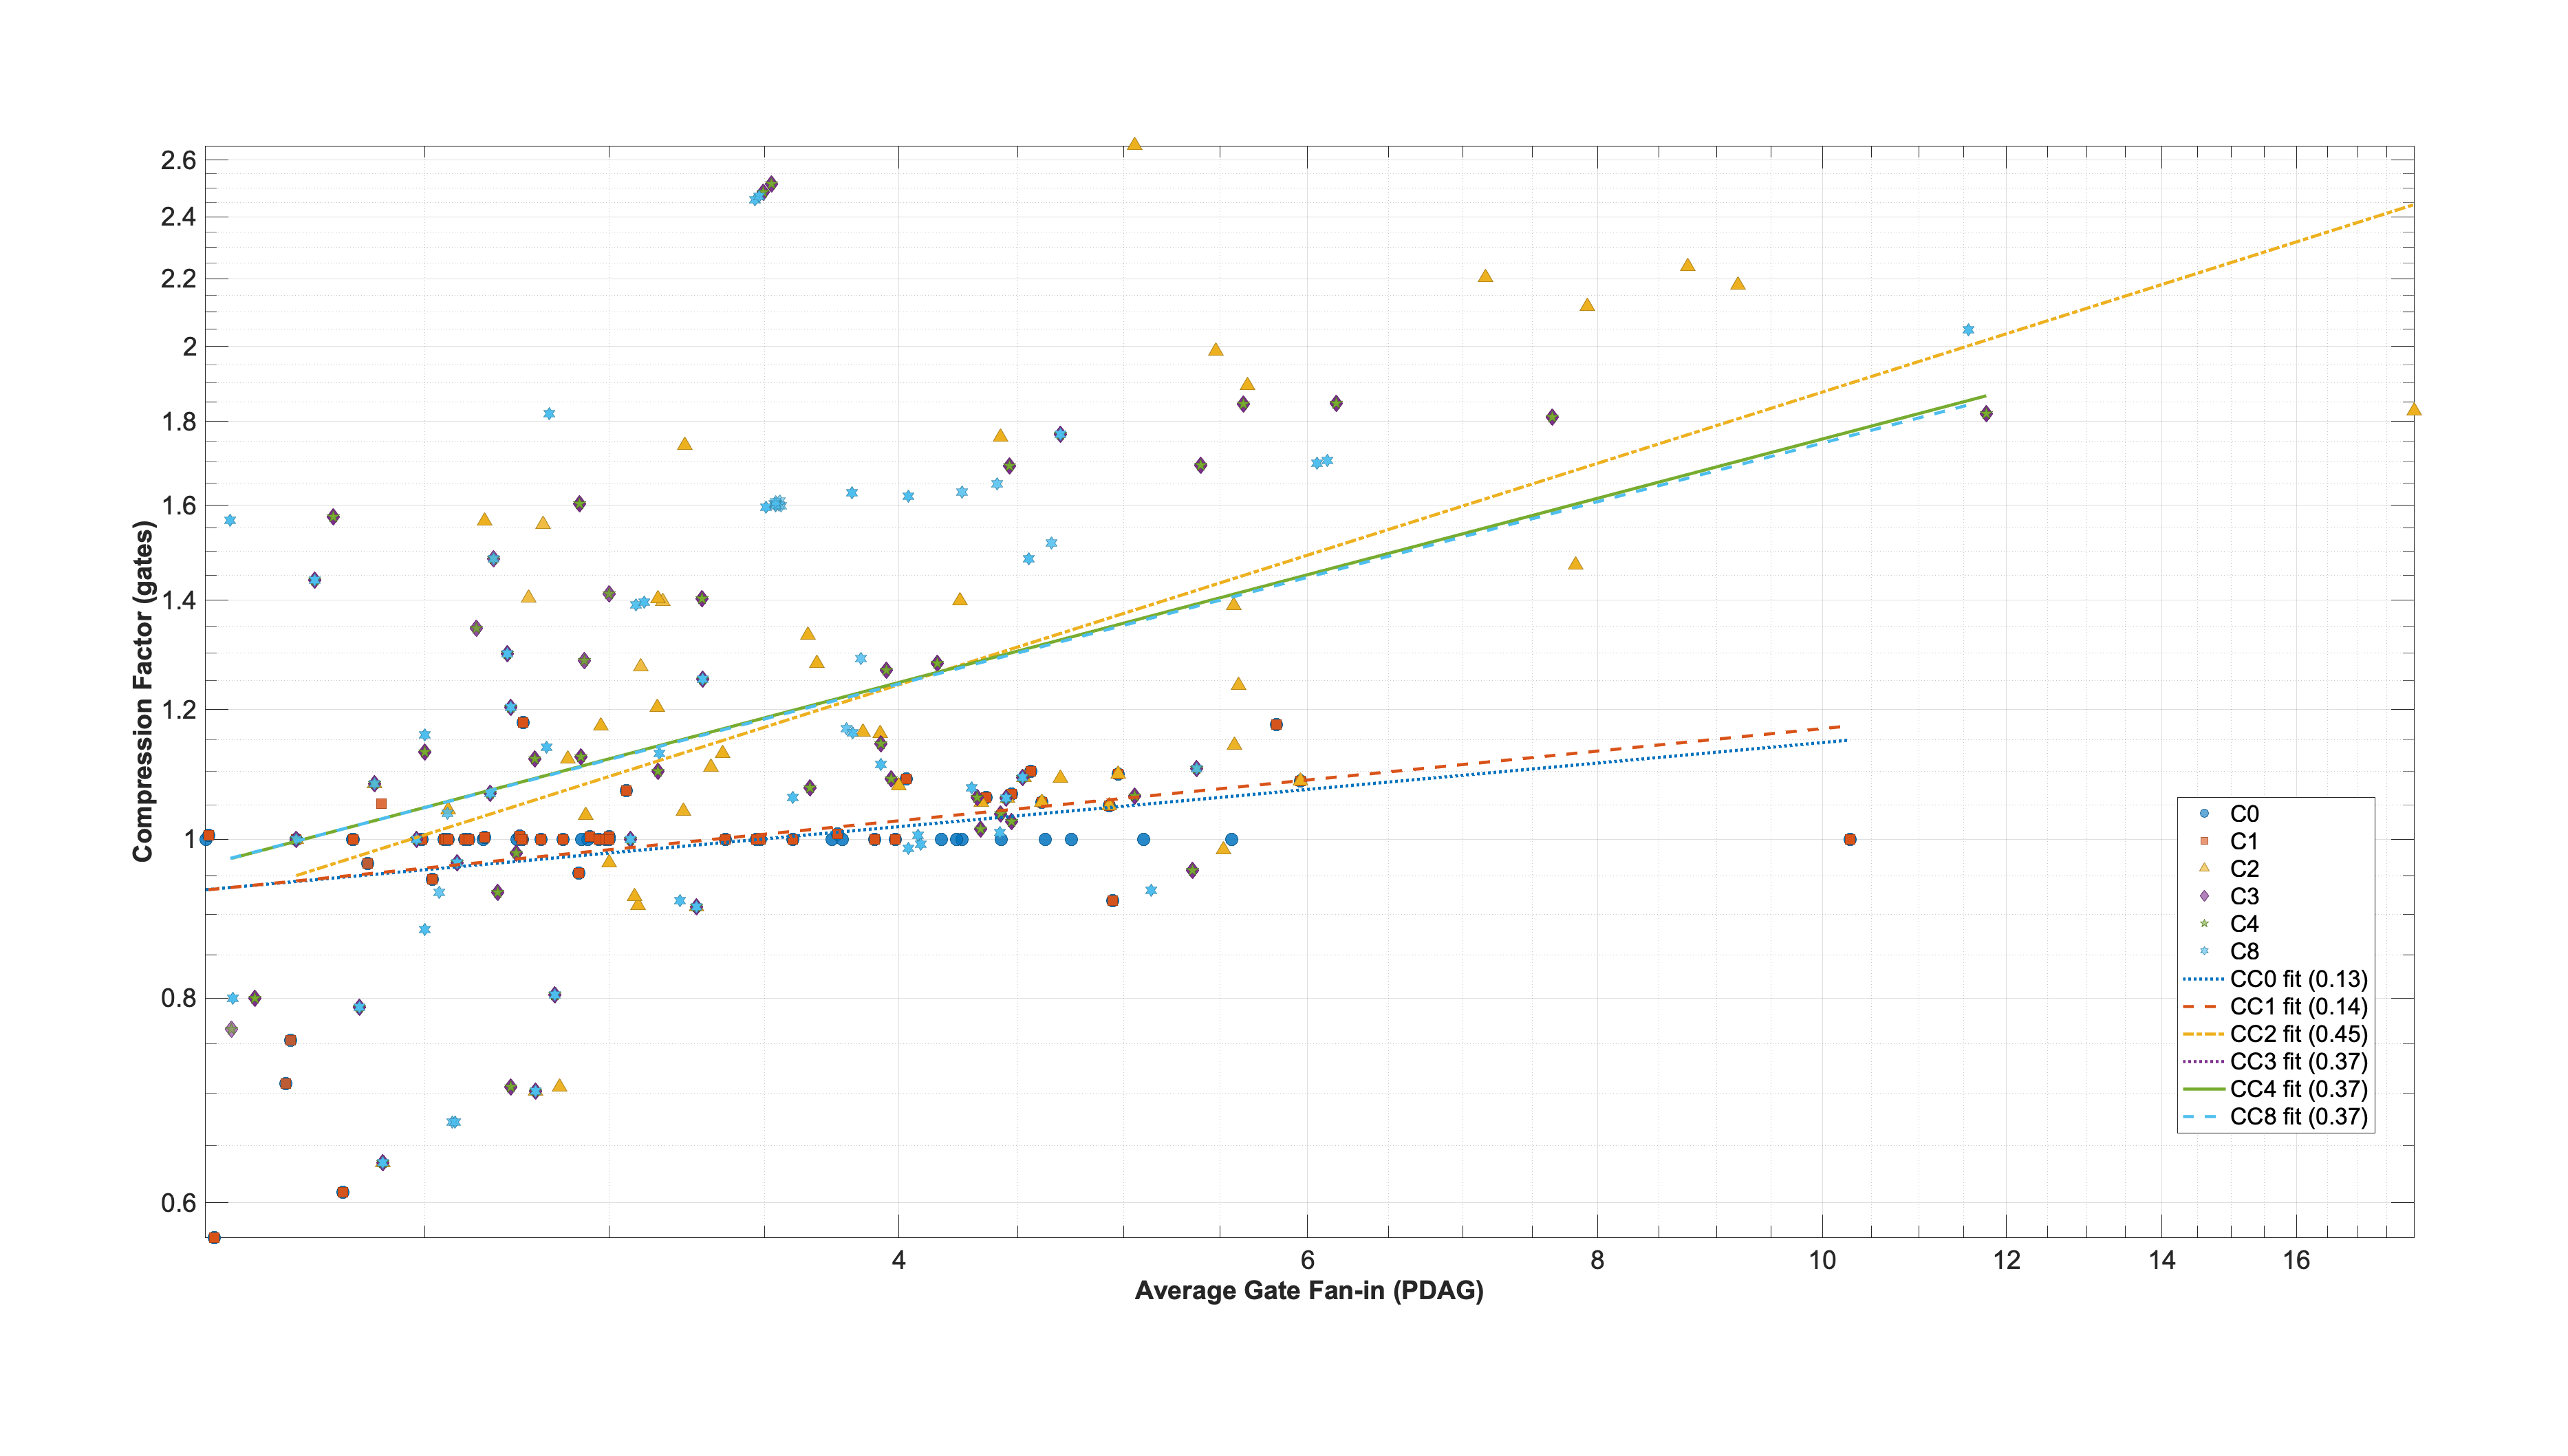
\includegraphics[width=1.15\textwidth]{figs/compiler/compiler_fanin_vs_compression.png}
    \caption{Relationship between average gate fan-in $f$ in the compiled PDAG and structural compression factor $\gamma$.  Points are colored by compilation flag; dashed lines show ordinary least–squares fits on log--log axes with slopes indicated in the legend.}
    \label{fig:compiler_fanin_compression}
\end{figure}
\end{landscape}

Pooling all compilation levels, the relationship between compression
and average gate fan-in $f$ is well described by the log–log regression

\[
  \log_{10}\gamma \;=\; 0.370\,\log_{10}f \; - \; 0.128,
  \qquad R^{2}=0.17\;(n=2064).
\]
Equivalently
$\gamma\approx0.75\,f^{0.37}$, indicating sub-linear returns: doubling
average fan-in improves compression by only $29\%$.

\begin{table}[t]
  \centering
  \caption{Global regression of compression factor on average fan-in.}
  \label{tab:micro_fanin_global}
  \begin{tabular}{lcccc}
    \toprule
    Dataset & Slope $a$ & Intercept $b$ & $R^{2}$ & $n$ \\
    \midrule
    All models & 0.370 & $-0.128$ & 0.17 & 2064 \\
    \bottomrule
  \end{tabular}
\end{table}

The modest $R^{2}$ reflects structural heterogeneity among models: in
series–parallel fragments compression saturates regardless of $f$,
whereas highly redundant safety logic with large voting constructs
exhibits super-linear sharing potential.  A finer taxonomy of these
architectures remains future work.
